\documentclass[11pt]{article}


\usepackage{fullpage}
\usepackage{graphicx}
\usepackage{amsmath}
\usepackage{amssymb}
\usepackage{amsthm}
\usepackage{fancyvrb}

\newcommand{\myname}{Mehshan Mustafa}

\newenvironment{theorem}[2][Theorem]{\begin{trivlist}
\item[\hskip \labelsep {\bfseries #1}\hskip \labelsep {\bfseries #2.}]}{\end{trivlist}}
\newenvironment{lemma}[2][Lemma]{\begin{trivlist}
\item[\hskip \labelsep {\bfseries #1}\hskip \labelsep {\bfseries #2.}]}{\end{trivlist}}
\newenvironment{exercise}[2][Exercise]{\begin{trivlist}
\item[\hskip \labelsep {\bfseries #1}\hskip \labelsep {\bfseries #2.}]}{\end{trivlist}}
\newenvironment{problem}[2][Problem]{\begin{trivlist}
\item[\hskip \labelsep {\bfseries #1}\hskip \labelsep {\bfseries #2.}]}{\end{trivlist}}
\newenvironment{question}[2][Question]{\begin{trivlist}
\item[\hskip \labelsep {\bfseries #1}\hskip \labelsep {\bfseries #2.}]}{\end{trivlist}}
\newenvironment{corollary}[2][Corollary]{\begin{trivlist}
\item[\hskip \labelsep {\bfseries #1}\hskip \labelsep {\bfseries #2.}]}{\end{trivlist}}
\newenvironment{solution}{\begin{proof}[Solution]}{\end{proof}}
\newenvironment{idea}[2][Proof Idea.]{\textit{#1} #2}



\parindent0in
\pagestyle{plain}
\thispagestyle{plain}

\usepackage{csquotes}
\usepackage[shortlabels]{enumitem}

\newcommand{\dated}{\today}
\newcommand{\token}[1]{\langle \text{#1} \rangle}

\begin{document}

\textbf{Introduction to the Theory of
Computation}\hfill\textbf{\myname}\\[0.01in]
\textbf{Chapter 7: Time Complexity}\hfill\textbf{\dated}\\
\smallskip\hrule\bigskip

\begin{problem}{7.15}
Show that P is closed under the star operation.
\end{problem}
\begin{idea}
For any language $A \in P$, a string $y = y_1 \cdots y_n \in A^{*}$, when one of following is true:
\begin{enumerate}
\item $y = \varepsilon$.
\item $y \in A$.
\item Both sub-strings of one of possible splits of $y$ are in $A^{*}$.
\end{enumerate}
\begin{center}
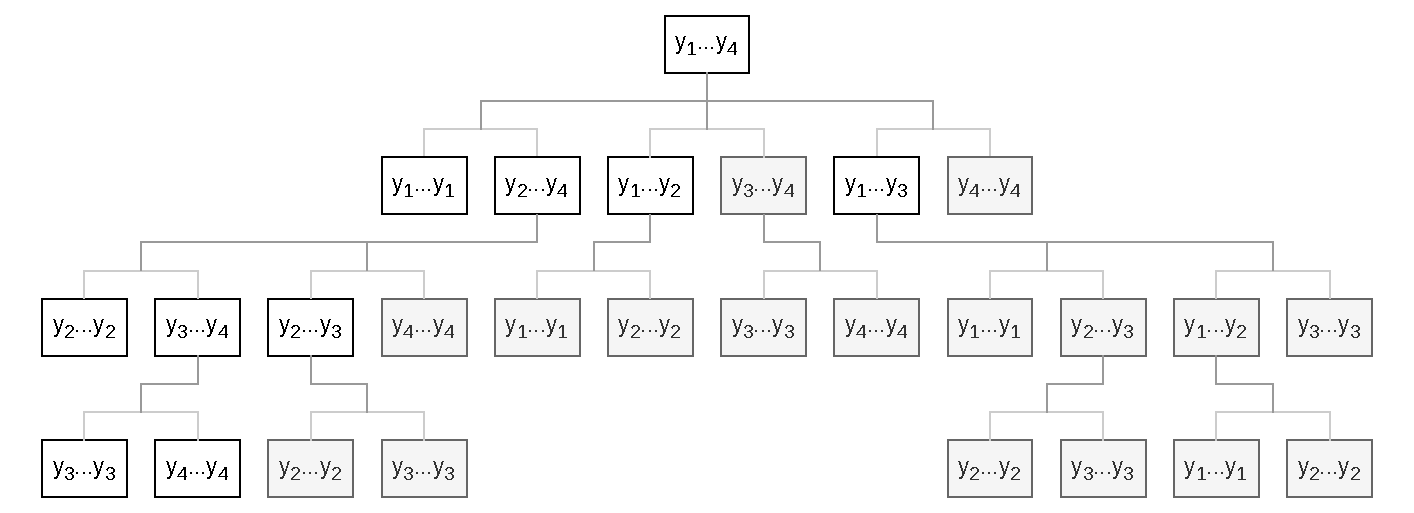
\includegraphics[scale=0.60]{Figures/Problem7.15a.pdf} \\
Tree of sub-problems for a string of length 4. \\
Non-shaded sub-problems are unique, whereas shaded are duplicate.
\end{center}
First, we give a recurive algorithm $C$ that tests if $A^{*}$ contains a string $y$. Secondly, we use \textit{Dynamic Programming} (recursion + memoinzation) to obtain a polynomial time algorithm $D$.
\end{idea}

\begin{proof}Let $A$ be any language in $P$ and $T$ be the \textbf{TM} that decides $A$ in polynomial time. \\

$C =$ \textquotedblleft On input $\langle y, i, j \rangle$, where $y$ is a string and $i, j$ are integers:
\begin{enumerate}
\item If $y = \varepsilon$, then \textit{accept}.
\item Use $T$ to check if $y_i \cdots y_j \in A$. If $T$ accepts, then \textit{accept}.
\item Repeat for each $k$ between $i+1$ and $j$.
\item \hspace*{0.5cm} Run $C$ on $\langle y, i, k - 1 \rangle$.
\item \hspace*{0.5cm} Run $C$ on $\langle y, k, j \rangle$.
\item \hspace*{0.5cm} \textit{Accept}, if $C$ accepts in both cases.
\item \textit{Reject}.\textquotedblright
\end{enumerate}
Then decide $A^{*}$ by starting with $i=1$ and $j=|y|$.

$D =$ \textquotedblleft On input $\langle y, i, j \rangle$, where $y$ is a string and $i, j$ are integers:
\begin{enumerate}
\item If $y = \varepsilon$, then \textit{accept}.
\item If previously solved then answer same, else continue.
\item Use $T$ to check if $y_i \cdots y_j \in A$. If $T$ accepts, then \textit{accept}.
\item Repeat for each $k$ between $i+1$ and $j$.
\item \hspace*{0.5cm} Run $C$ on $\langle y, i, k - 1 \rangle$.
\item \hspace*{0.5cm} Run $C$ on $\langle y, k, j \rangle$.
\item \hspace*{0.5cm} \textit{Accept}, if $C$ accepts in both cases.
\item \textit{Reject}.\textquotedblright
\end{enumerate}
Then decide $A^{*}$ by starting with $i=1$ and $j=|y|$.

\begin{center}
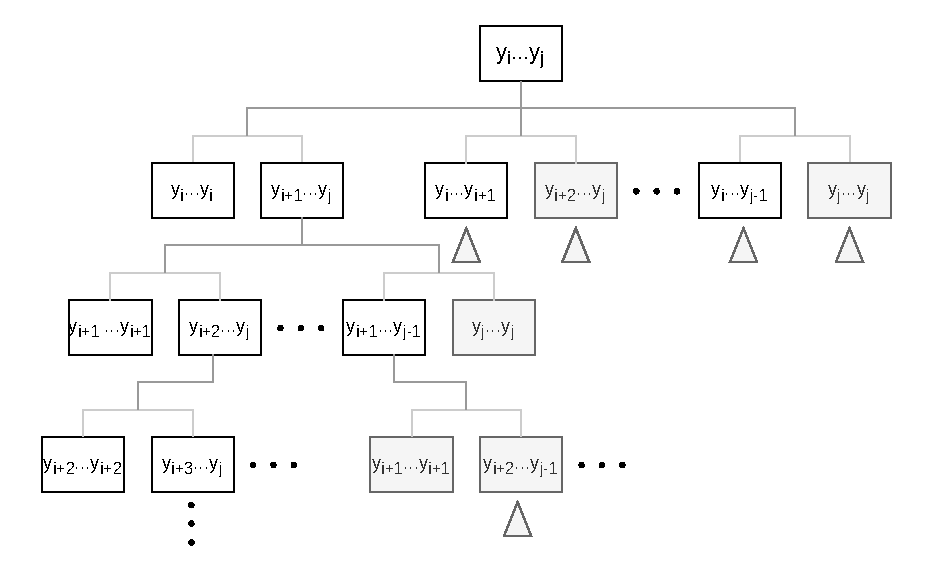
\includegraphics[scale=1.0]{Figures/Problem7.15b.pdf} \\
Tree of sub-problems for a string $y = y_i \cdots y_j$. \\
Shaded sub-problems are duplicate.
\end{center}

\end{proof}

\end{document}